\begin{frame}
	\frametitle{Hydrosphäre - Wassermassen}
	\begin{figure}
		\centering
		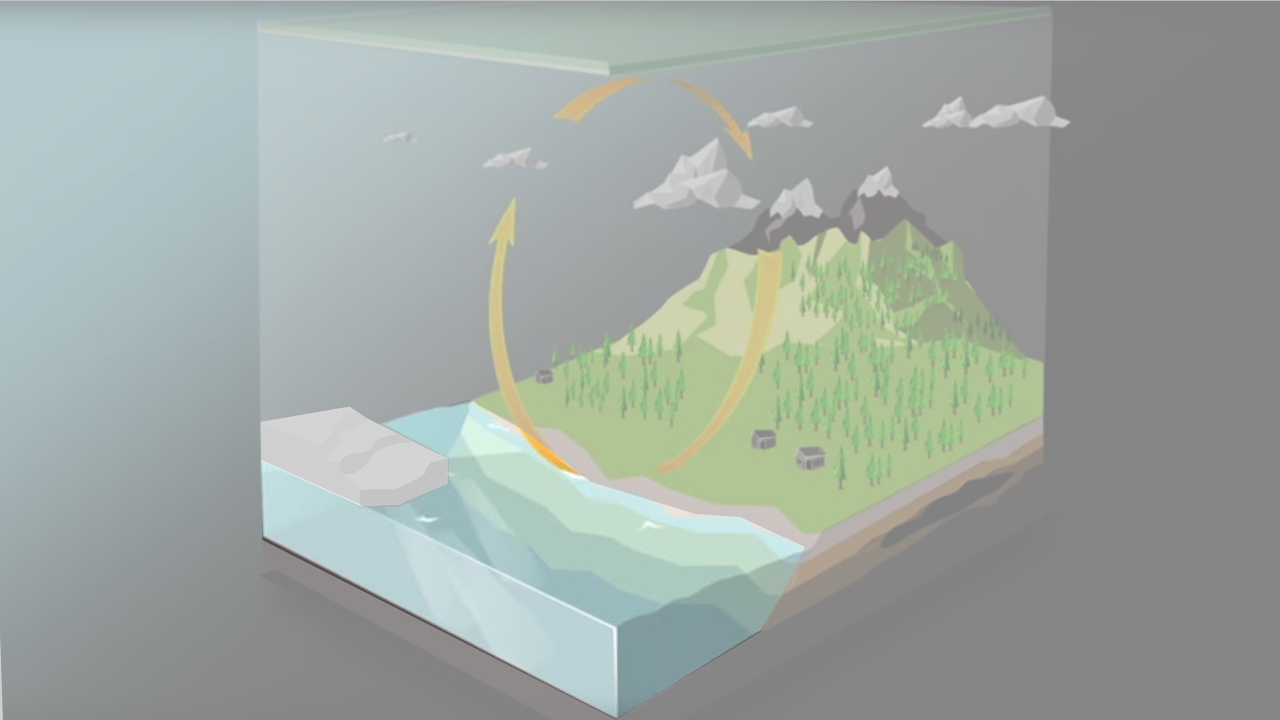
\includegraphics{bilder/WMO_Cycles_water.png}
		\caption{Etwa 2/3 der Erdoberfläche sind von Wasser bedeckt, somit ist die Hydrosphäre allein durch die Masse ein wichtiger Faktor des Klimasystems.}
	\end{figure}

	\note{
	\begin{itemize}
		\item[] Etwa 2/3 der Erdoberfläche sind von Wasser bedeckt, somit ist die Hydrosphäre allein durch die Masse ein wichtiger Faktor des Klimasystems.
		\item[] Daher widmen wir uns zuerst den Wassermassen.
		% Aufteilung von https://www.lenntech.de/faq-wasser-menge.htm, aber auch Wetzel, Robert G. 1983 in "Periphyton of freshwater ecosystems"
    \item[] Der Großteil der Wassermassen ist Salzwasser 97\,\%.
    \item[] Süßwasser (Flüsse und Seen) bildet nur weniger als 1\,\% des globalen Wassers.
    \item[] Eismassen machen ca. 2\,\% des Wassers aus und binden den größten Teil des Süßwassers, da das Salz bei der Eisbildung im Wasser gelößt bleibt.
    \item[] Eis betrachten wir später.
	\end{itemize}
	}
\end{frame}


\begin{frame}
	\frametitle{Eigenschaften des Wassers} % M.Latif Klimawandel und Klimadynamik S. 23
	\begin{itemize}
		\item Wasser ist ein Dipol-Molekül \textcolor{blue}{H$_2$O}
		\begin{itemize}
			\item[$\rightarrow$] Kann wirksam Infrarotstrahlung absorbieren
			\item[$\rightarrow$] Kann viel Wärme aufnehmen bevor es verdampft $\rightarrow$ "Trägheit"
		\end{itemize}

		%Allgemein liegt die größte Dichte des Wassers bei 4 Grad
		\item<2-> Größte Dichte von reinem Wasser bei \SI{4}{°C}
		\begin{itemize}
			\item<2->[$\rightarrow$] Eis schwimmt auf Wasser
		\end{itemize}
		% Im besonderen Fall des Salzwassers liegt die größte Dichte jedoch bei -3.8 Grad
		\item<3->Größte Dichte von Salzwasser bei \SI{-3,8}{°C}
		\begin{itemize}
			\item<3-> [] Bei der Eisbildung wird verbleibt das Salz gelößt im Wasser
			\item<3-> [$\rightarrow$] Salzwasser kann kälter werden als Eis und sinkt in die tieferen Schichten des Ozeans
			\item<3-> [$\rightarrow$] Wärmeres, weniger dichtes Wasser steigt auf
			\item<3-> [] \textbf{\textcolor{blue}{Konvektion}} in den Polarregionen
			\item<3-> [$\rightarrow$] Kohlenstoffsenken
		\end{itemize}
	\end{itemize}

	\note{
		\begin{itemize}
      \item[] Wasser ist ein Dipol-Molekül
			\item[] Wärmekapazitäten im Vergleich
			\begin{itemize}
				\item[] Wasserstoff (Gas) \SI{14,3}{J\per g\per K}
				\item[] Helium (Gas) \SI{5,2}{J\per g\per K}
				\item[] Ammoniak (Flüssigkeit) \SI{4,7}{J\per g\per K}
				\item[] Lithium (Flüssigkeit) \SI{4,4}{J\per g\per K}
				\item[] Wasser (Flüssigkeit) \SI{4,2}{J\per g\per K}
			\end{itemize}
			\item[] Das Phänomen Konvektion ist nicht auf Wasser beschränkt. Gibt es auch in der Luft oder wird durch Pumpen erzeugt.
			\item[] die Konvektion ist durch die temperaturbedingte Dichte und den Salzgehalt möglich
			\item[] daher auch unter dem Namen \textit{thermohaline Konvektion} (thermo - Temperatur, halin - Salz) bekannt
			\item[] Oberflächen nahes, Kohlenstoff reiches Wasser wird abgesenkt $\rightarrow$ Kohlenstoffsenken
		\end{itemize}
	}

% TODO: evtl. Abbildung der Konvektion: Abgabe von Wärme bei Aufnahme von atmosphärischen Gasen, die dann in die Tiefsee gelangen und dort gespeichert werden

%TODO: Erklärung von Senken
\end{frame}

\begin{frame}
	\frametitle{Wasserdynamik} %M. Latif Klimawandel und Klimadynamik S.24
	\begin{figure}
    \centering
    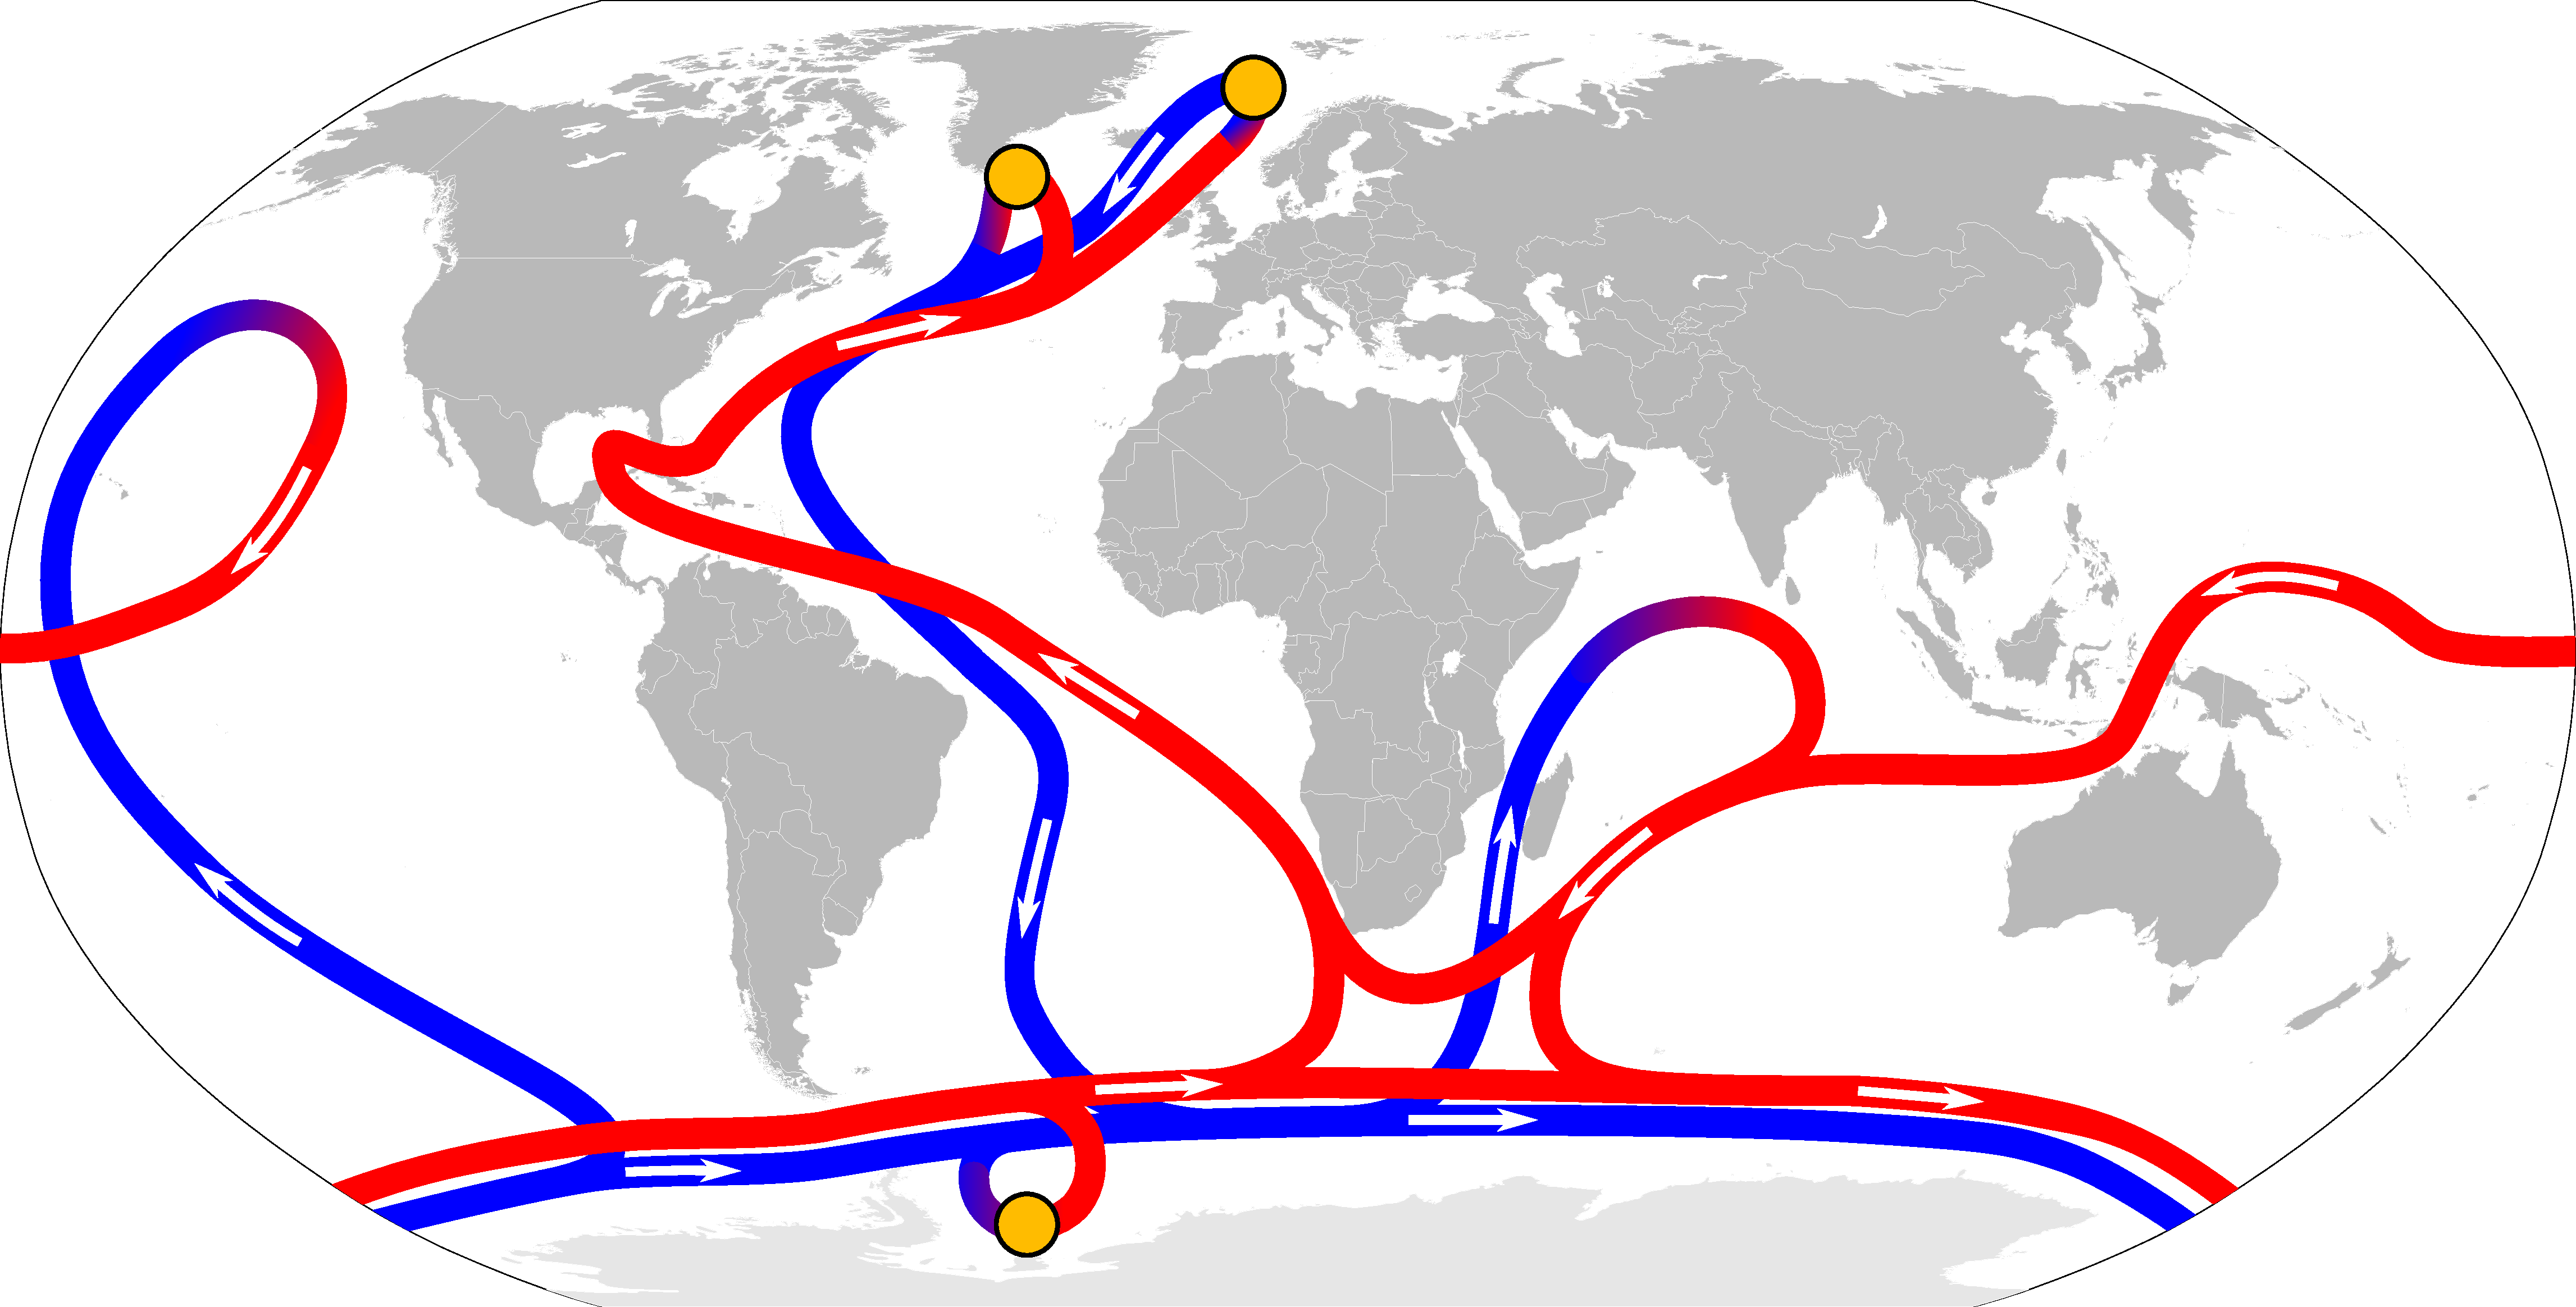
\includegraphics[width=.9\linewidth]{bilder/Thermohaline_Circulation.pdf}
    \caption{Termohaline Zirkulation, Quelle: nach Robert Simmon, NASA}
  \end{figure}

	\note{
		\begin{itemize}
			\item[] Die großen Wassermassen der Ozeane haben eine bestimmte Strömung, z.B. Golfstrom von der Arktis über die Küste Mexikos bis an die Antarktis.
			\item[] Die Stömung ergibt sich vorallem durch die Erdrotation (Corioliskraft).
			\item[] Die oberflächliche Strömung der oberen 100 Meter entsteht durch Wind (und darauf resultierende Reibung) und die Form der Meeresbecken.
			\item[] Die Tiefenströmung wird durch die Konvektion angetrieben. Die Dichte des Wassers spielt dabei eine entschiedende Rolle, da dichteres Wasser nach unten sinkt und leichteres empor steigt.
			\item[] Warme Temperaturen führen zum aufwärmen des Oberflächenwassers und damit zu einer geringeren Dichte.
			\item[] Dadurch werden Oberflächenwasser und Tiefenwasser stark getrennt - und somit strömen die Wassermassen mit unterschiedlicher Geschwindigkeit.
      \item[] Unterscheidung zwischen zwei Zirkulationen
      \begin{itemize}
        \item[Windgetrieben] Oberflächenströmung der Ozeane durch Reibung, Erdrotation (Corioliskraft) und Form der Meeresbecken, eher horizontal
        \item[Dichtegetrieben] Erwärmung, Abkühlung, und Änderung des Salzgehaltes (durch Eisbildung, Verdunstung oder Niederschlag) haben Einfluss auf die Dichte des Wassers, wodurch die Wassermassen zirkulieren, eher vertikal
      \end{itemize}
		\end{itemize}
	}

\end{frame}


\begin{frame}
	\frametitle{Wirkung des Wassers auf das Klima}
	\begin{itemize}
	\item Ca. 70\,\% der Erdoberfläche ist mit Wasser bedeckt
	\item [$\rightarrow$] Die \textit{Trägheit} des Wassers ist ein entscheidender Faktor für die Trägheit des Klimas und der Klimaänderungen % M.Latif Klimawandel und Klimadynamik S. 23
	\item Kohlenstoffsenken in der Tiefsee können durch erwärmen der Ozeane \textit{irgendwann} freigesetzt werden
	\item[$\rightarrow$] massiver Anstieg des atmosphärischen CO$_2$ $\rightarrow$ Verstärkung des Treibhauseffekts
	\item Positive Verstärkung von CO$_2$ und Wasserdampf: eine wärmere Atmosphäre kann mehr Wasserdampf (und CO$_2$) aufnehmen (Eis-Albedo-Rückkopplung)
	\end{itemize}
\end{frame}

\begin{frame}
	\frametitle{Trägheit des Klimas}
	\begin{figure}
		\centering
		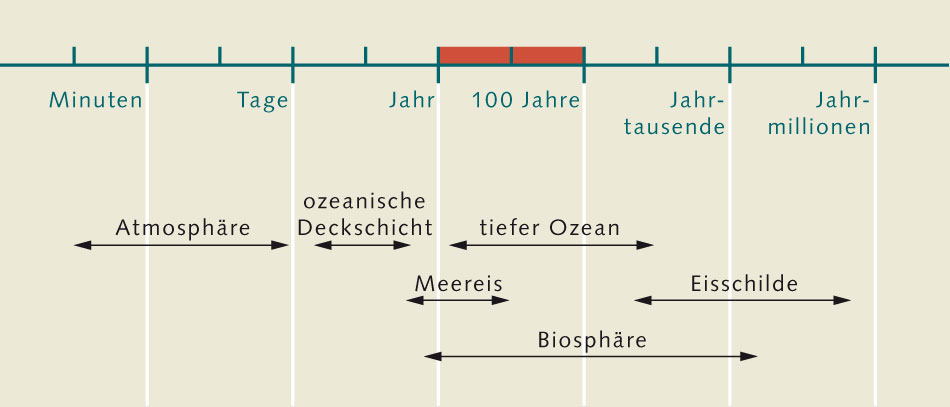
\includegraphics[width=0.8\linewidth]{bilder/zeitskala-klimasystem_world_ocean_review.jpg}
		\caption{Zeitskalen im Klimasystem, Quelle: maribus nach Meinecke und Latif, 1995}
		\label{fig:traegheit}
	\end{figure}

  \begin{itemize}
    \item[$\rightarrow$] Verzögertes Feedback bis zu einem klimawirksamen Ereignis.
    \item[$\rightarrow$] Besonders die Ozeane und Eisschilde benötigen eine sehr lange Zeit, um sich geänderten klimatischen Bedingungen anzupassen.
  \end{itemize}

	\note{
		\begin{itemize}
			\item[] Trägheit des Wassers ist entscheident.
			\item[] Die Wassermassen sind in dieser Abbildung stark vertreten.
			\item[] Die untere Atmosphäre passt sich innerhalb weniger Stunden den Bedingungen der Erdoberfläche an (Temeperatur, Gase, etc.)
			\item[] Die Wassermassen reagieren sehr unterschiedlich.
			\item[] Flüsse, Seen und Oberflächenwasser wärmen sich dabei deutlich schneller auf als die tieferen Ozeanschichten. (Das kennt man vielleicht aus Bade- oder Bergseen - die oberen 50 cm sind angenehm warm und darunter liegt deutlich kälteres Wasser)
			\item[] Besonders unterschiedlich schnell reagiert die Biosphäre.
      \begin{itemize}
        \item[] Graslandschaften können schnell austrocken
        \item[] Wälder dagegen verändern sich über Jahrtausende hinweg.
        \item[] Die Vegetation bestimmt in vielen Fällen auch die Ansiedlung von Lebewesen.
        \item[] Die Änderung der Vegetation kann das Ende des Lebenraums einiger Lebewesen bedeuten, aber auch neue Ansiedluneg bedingen.
      \end{itemize}
			\item[] Eine besonders lange Reaktionszeit haben die Eisschilde der Erde. Auf die Eismassen gehen wir als nächstes ein.
		\end{itemize}
	}
\end{frame}
